% !TEX encoding = UTF-8 Unicode
% !TEX TS-program = pdflatex

% toptesti document class
\documentclass[%
    a4paper, % not needed, by default it is a4paper, or also b5paper can be used
    corpo=12pt, % dimension of basic font
    % oneside is generally the way to go
    twoside, % two side optimizes for two-face printing, having chapters open on the right (aka odd numbers), if you don't want blank pages put oneside here
    stile=standard,
    %evenboxes, % not needed, to put supervisors and candidate at the same level
    tipotesi=magistrale,
    % numerazioneromana, % roman numbering for appendixes and preambles, up to Table of Contents
    openright, % to force opening on the right for double-sided printing
    cucitura=7mm, % for printing, 7mm should be enough
    %dvipsnames, % for compatibility with xcolor, it does not work
]{toptesi}

%%%%%%%%%%%%%%%%%%%%%%%%%%%%%%%%%%%%%%%%%%%%%%%%%%%%
\usepackage[english]{babel}
\usepackage[utf8]{inputenc}
\usepackage[T1]{fontenc}
\usepackage{lmodern}
% bibliography
\usepackage[hyperref=true,backref=true,backend=biber,maxbibnames=9,maxcitenames=2,style=ieee,citestyle=numeric,sorting=none]{biblatex}
% Customizing backref output
\DefineBibliographyStrings{english}{
    backrefpage = {\thefield{backref}}, % Formatting for single backref
    backrefpages = {\thefield{backref}}  % Formatting for multiple backrefs
}
% Adjusting the format of back-references
\renewbibmacro*{pageref}{%
    \iflistundef{pageref}
    {}
    {\printtext[brackets]{%
            \printlist{pageref}}}}
\renewbibmacro*{finentry}{%
    \iffieldundef{pageref}
    {}
    {\addspace\printtext[brackets]{\printlist{pageref}}}%
    \finentry}
% Redefine \cite to make text and number black
\usepackage{xcolor} % for color
\usepackage{etoolbox}
\usepackage{hyperref} % for hyperlinks
\makeatletter
\let\oldcite\cite
\AtBeginDocument{
    \renewcommand{\cite}[1]{\textcolor{black}{\hypersetup{citecolor=black}\oldcite{#1}}}
}
\makeatother

\usepackage{adjustbox} % to resize boxes by keeping the same aspect ratio
\usepackage{algorithm} % algorithm environment
\usepackage{algpseudocode} % improved pseudo-code
\usepackage{amsfonts}               %  AMS mathematical fonts
\usepackage{amsmath}
\usepackage{amssymb}                %  AMS mathematical symbols
\usepackage{bm}                     %  black/bold mathematical symbols
\usepackage{booktabs}               %  better tables
\usepackage[labelfont=bf]{caption} % font=footnotesize % to have reduced caption font size
\usepackage{csquotes}
\usepackage{enumitem} %left align the bulleted points
\usepackage{geometry} % FOR DEBUG USE [showframe]{geometry}
%\usepackage{glossaries} % to use acronyms and glossary, it has also glossaries-extra as extension, but commands are different
\usepackage[%
    toc, % puts the link in the ToC
    %record, % to use bib2gls
    abbreviations, % to load abbreviations / acronyms
    nonumberlist, % to avoid printing the numbers of the references in the acronyms page
]{glossaries-extra}
\usepackage{graphicx}               %  post-script images
\usepackage{wrapfig}
%\usepackage{iwona} % extra fonts, substitute standard ones
\usepackage{layout} % debug
\usepackage{listings} % to insert formatted code
\usepackage{lipsum} % for lorem ipsum text, not needed in the real work
\usepackage{makecell} % to change dimensions of cells, for math cases
\usepackage{mathtools} % for additional commands
\usepackage{mfirstuc} % to have capitalization capabilities
\usepackage[final]{microtype}      % microtypography, final lets latex use it also in bibliography
\usepackage{setspace} % for line spacing
\usepackage{multirow} % to allow for cells covering more than 1 row in tables
\usepackage{nicefrac}       % compact symbols for 1/2, etc.
%\usepackage[lofdepth,lotdepth]{subfig}
\usepackage{ragged2e} % for justifying text
\usepackage{rotating} % rotates things
\usepackage{siunitx} % support for SI units of measurement and number typesetting
\usepackage{subfig}
\usepackage{svg} % for svg support, works only if inkscape is installed, default for Overleaf v2
%\usepackage{subfigure}              %  subfigure compatibility, can be removed if subfig
\usepackage{tabularx} % equal-width columns in tables
\usepackage{textcomp} % extra fonts and symbols
\usepackage{url}            % simple URL typesetting
\usepackage{verbatim} % for extended verbatim support
\usepackage{xcolor} % to define colors and use standard CSS names add dvipsnames as option, but it clashes with xcolor loaded in toptesi, pay attention that if it goes in conflict with tikz/beamer, simply use \documentclass[usenames,dvipsnames]{beamer}, along with other custom options when defining the document class
\usepackage{xifthen}
\usepackage[nottoc]{tocbibind}
\usepackage{placeins}
\usepackage{hyperref} % must be loaded before glossaries-extra
\usepackage{cleveref}

% ------------------ \cref REDEFINITION with black color (only link now) -----------------------------
% ------------------ NORMAL -----------------------------
\crefformat{figure}{
    \unskip\textcolor{black}{ % fig. text color
        fig.~#2\textcolor{black}{#1}#3} % reference number color
    \unskip
}
\crefformat{table}{
    \unskip\textcolor{black}{ % table text color
        table~#2\textcolor{black}{#1}#3} % reference number color
    \unskip
}
\crefformat{section}{
    \unskip\textcolor{black}{ % section text color
        section~#2\textcolor{black}{#1}#3} % reference number color
    \unskip
}
\crefformat{equation}{
    \unskip\textcolor{black}{ % equation text color
        eq.~#2\textcolor{black}{#1}#3} % reference number color
    \unskip
}
% ------------------ CAPITALIZED -----------------------------
\Crefformat{figure}{
    \unskip\textcolor{black}{ % Fig. text color
        Fig.~#2\textcolor{black}{#1}#3} % reference number color
    \unskip
}
\Crefformat{table}{
    \unskip\textcolor{black}{ % Table text color
        Table~#2\textcolor{black}{#1}#3} % reference number color
    \unskip
}
\Crefformat{section}{
    \unskip\textcolor{black}{ % Section text color
        Section~#2\textcolor{black}{#1}#3} % reference number color
    \unskip
}
\Crefformat{equation}{
    \unskip\textcolor{black}{ % Eq. text color
        Eq.~#2\textcolor{black}{#1}#3} % reference number color
    \unskip
}

% configuration for glossaries
% convert and load converted glossaries in .tex ,format from .bib
\setabbreviationstyle{long-short-desc} % style before loading resources
% this command sets the style to title for long names of acronyms only in the glossary description, leading to capitalized first-letter for all words
% \glssetcategoryattribute{\glsxtrabbrvtype}{glossname}{capitalisewords} % doesn't work
% resources to load if using a bib file with bib2gls
%\GlsXtrLoadResources[%
% src={glossaries}, % name of the file without extension
% selection=all, % select all the entries
%]
% not needed
%\newglossary*{abbreviation}{Acronyms} % to change the name of this glossary for acronyms

%\renewcommand{\glsclearpage}{\paginavuota} % to allow glossaries to clear pages, done manually is better


% setup for hyperref
\hypersetup{%
    pdfpagemode={UseOutlines},
    bookmarksopen,
    pdfstartview={FitH},
    pdftitle={ThesisTitle},
    pdfauthor={Matteo Minotti},
    colorlinks,
    linkcolor={black}, % it is suggested to keep them black, since when printing it it costs per page, and if they have color it's twice the price per page
    citecolor={black},
    urlcolor={black}
  }
%

% setup for svg
\svgsetup{%
    inkscapeformat=pdf, % to force usage of PDF
    inkscapelatex=false, % to disable latex rendering of text, produces errors
}

% setup for siunitx, it does not work in the summary
\sisetup{%
    detect-all, % to use the same font as for writing when using \num
    mode=text, % to allow it to work also in math mode
    group-separator = {,}, % separator for number grouping
    group-minimum-digits = 3, % minimum number of digits a number must have to be grouped in 3-digit groups
}

% listings colours
\definecolor{rulecolor}{rgb}{0,0,0}
\definecolor{commentcolor}{rgb}{0,0.6,0}
\definecolor{linenumbercolor}{rgb}{0.5,0.5,0.5}
\definecolor{keywordcolor}{rgb}{0,0,0.95}
\definecolor{backcolor}{rgb}{1,1,1}%{0.95,0.95,0.92}
\definecolor{stringcolor}{rgb}{0.58,0,0.82}

% setup for lstlisting
\lstset{ %
	backgroundcolor=\color{backcolor},   % choose the background color; you must add \usepackage{color} or \usepackage{xcolor}; should come as last argument
	basicstyle=\footnotesize,        % the size of the fonts that are used for the code
	breakatwhitespace=false,         % sets if automatic breaks should only happen at whitespace
	breaklines=true,                 % sets automatic line breaking
	captionpos=t,                    % sets the caption-position to bottom
	commentstyle=\color{commentcolor},    % comment style
	extendedchars=true,              % lets you use non-ASCII characters; for 8-bits encodings only, does not work with UTF-8
	frame=single,	                   % adds a frame around the code
	keepspaces=true,                 % keeps spaces in text, useful for keeping indentation of code (possibly needs columns=flexible)
	keywordstyle=\color{keywordcolor},       % keyword style
	%language=VHDL,                 % the language of the code
	numbers=left,                    % where to put the line-numbers; possible values are (none, left, right)
	numbersep=5pt,                   % how far the line-numbers are from the code
	numberstyle=\tiny\color{linenumbercolor}, % the style that is used for the line-numbers
	rulecolor=\color{rulecolor},         % if not set, the frame-color may be changed on line-breaks within not-black text (e.g. comments (green here))
	showspaces=false,                % show spaces everywhere adding particular underscores; it overrides 'showstringspaces'
	showstringspaces=false,          % underline spaces within strings only
	showtabs=false,                  % show tabs within strings adding particular underscores
	stepnumber=1,                    % the step between two line-numbers. If it's 1, each line will be numbered
	stringstyle=\color{stringcolor},     % string literal style
	tabsize=4,	                   % sets default tabsize to 2 spaces
	title=\lstname,                   % show the filename of files included with \lstinputlisting; also try caption instead of title
	inputencoding=utf8,
	literate=
	{á}{{\'a}}1 {é}{{\'e}}1 {í}{{\'i}}1 {ó}{{\'o}}1 {ú}{{\'u}}1
	{Á}{{\'A}}1 {É}{{\'E}}1 {Í}{{\'I}}1 {Ó}{{\'O}}1 {Ú}{{\'U}}1
	{à}{{\`a}}1 {è}{{\`e}}1 {ì}{{\`i}}1 {ò}{{\`o}}1 {ù}{{\`u}}1
	{À}{{\`A}}1 {È}{{\'E}}1 {Ì}{{\`I}}1 {Ò}{{\`O}}1 {Ù}{{\`U}}1
	{ä}{{\"a}}1 {ë}{{\"e}}1 {ï}{{\"i}}1 {ö}{{\"o}}1 {ü}{{\"u}}1
	{Ä}{{\"A}}1 {Ë}{{\"E}}1 {Ï}{{\"I}}1 {Ö}{{\"O}}1 {Ü}{{\"U}}1
	{â}{{\^a}}1 {ê}{{\^e}}1 {î}{{\^i}}1 {ô}{{\^o}}1 {û}{{\^u}}1
	{Â}{{\^A}}1 {Ê}{{\^E}}1 {Î}{{\^I}}1 {Ô}{{\^O}}1 {Û}{{\^U}}1
	{œ}{{\oe}}1 {Œ}{{\OE}}1 {æ}{{\ae}}1 {Æ}{{\AE}}1 {ß}{{\ss}}1
	{ű}{{\H{u}}}1 {Ű}{{\H{U}}}1 {ő}{{\H{o}}}1 {Ő}{{\H{O}}}1
	{ç}{{\c c}}1 {Ç}{{\c C}}1 {ø}{{\o}}1 {å}{{\r a}}1 {Å}{{\r A}}1
	{€}{{\euro}}1 {£}{{\pounds}}1 {«}{{\guillemotleft}}1
	{»}{{\guillemotright}}1 {ñ}{{\~n}}1 {Ñ}{{\~N}}1 {¿}{{?`}}1
}


% biblatex setup
% generally 9000 is ok, if higher than 10000 it's bad
% If you want to break on URL numbers
\setcounter{biburlnumpenalty}{9000}
% If you want to break on URL lower case letters
\setcounter{biburllcpenalty}{9000}
% If you want to break on URL UPPER CASE letters
\setcounter{biburlucpenalty}{9000}


\newcommand {\headerFont}[1]{\fontsize{16pt}{20pt}\selectfont{\textbf{#1}}}
\newcommand {\itemFont}[1]{\fontsize{10pt}{12pt}\selectfont{#1}}
% INTERLINEA E MARGINI
\newcommand {\myspacing}{1}
\edef\myleftmargin{2.5 cm}
\edef\myrightmargin{2.5 cm}

% change this configuration with your info
% if you need fewer or more supervisors you have to change \relatore command by adding or removing lines in the table in toptesi_config
\newcommand{\thesistitle}{TITLE}
\newcommand{\thesissubtitle}{} %
\newcommand{\thesisuniversitylogo}{images/logoPoliTo_with_name_2021} % choose your logo
\newcommand{\thesiscandidatename}{Name}
\newcommand{\thesiscandidatesurname}{SURNAME}
\newcommand{\thesissupervisoronetitle}{prof.}
\newcommand{\thesissupervisoronename}{Name}
\newcommand{\thesissupervisoronesurname}{SURNAME}
\newcommand{\thesissupervisortwotitle}{ing.}
\newcommand{\thesissupervisortwoname}{Name}
\newcommand{\thesissupervisortwosurname}{SURNAME}
\newcommand{\thesissupervisorthreetitle}{ing.}
\newcommand{\thesissupervisorthreename}{Name}
\newcommand{\thesissupervisorthreesurname}{SURNAME}
\newcommand{\thesisdate}{Month Year}
\newcommand{\thesisacademicyear}{202x/202x}

\newcommand{\thesiscommission}{Computer Engineering, Cinema and Mechatronics}
\newcommand{\thesisdept}{Control and Computer Engineering}
\newcommand{\thesiscourse}{Computer Engineering}
\newcommand{\thesisfield}{Automation and Intelligent Cyber-Physical Systems}
\newcommand{\thesisuniversity}{Politecnico di Torino}
\newcommand{\thesislevel}{Master} % master or bachelor
\newcommand{\thesiscandidatetext}{Candidate}
\newcommand{\thesissupervisortext}{Supervisors}


% fontsize is {size}{spacing}\family
\newcommand {\institutionfont}{\fontsize {22}{30}\scshape}
\newcommand {\divisionfont}{\fontsize {16}{20}\rmfamily}
\newcommand {\pretitlefont}{\fontsize {16}{16}\rmfamily}
\newcommand {\customtitlefont}{\fontsize {21}{28}\scshape}% {iwona}{bx}{n}}
\newcommand {\customsubtitlefont}{\fontsize {16}{20}\scshape}% {iwona}{bx}{n}}
\newcommand {\fixednamesfont}{\fontsize {14}{20}\mdseries}
\newcommand {\namesfont}{\fontsize {14}{20}\bfseries}
\newcommand {\footfont}{\fontsize {15}{18}\rmfamily}


\addbibresource{bibliography.bib}  

% Enable raggedbottom globally (text flow from the top to the bottom)
\raggedbottom

\begin{document}%\layout
% MARGIN SETUP
\newgeometry{left=\myleftmargin,right=\myrightmargin,top=\mytopmargin,bottom=\mybottommargin}

\english

\overfullrule=0.00001pt % latex shows a black bar for overfulls over this dimension

%\emergencystretch=1em % to allow some stretching in the lines to avoid overfull boxes, also in bibliography, eventually can be used only before bibliography or in the preamble for the whole document, not needed if using biblatex configuration in most cases


\ExtendCaptions{english}{Abstract}{Acknowledgements}

\ateneo{\thesisuniversity} % university name
\logosede[5cm]{\thesisuniversitylogo} % logo, square brackets contain the height

\titolo{\thesistitle} % title
%\sottotitolo{Metodo dei satelliti medicei} % subtitle

% place/remove a slash \\ to put the name on the following line or after Master Degree Course
\corsodilaurea{\thesiscourse} % course name


%~251197 % id number is not needed

\candidato{\thesiscandidatename~\textsc{\thesiscandidatesurname}} % candidate

% using tabular we can have more than 1 supervisor under the same column
\relatore{\tabular{@{}l}%
    \xmakefirstuc{\thesissupervisoronetitle}~\thesissupervisoronename~\textsc{\thesissupervisoronesurname}\\[0.4ex]
    \xmakefirstuc{\thesissupervisortwotitle}~\thesissupervisortwoname~\textsc{\thesissupervisortwosurname}\\[0.4ex]
    \xmakefirstuc{\thesissupervisorthreetitle}~\thesissupervisorthreename~\textsc{\thesissupervisorthreesurname}
    \endtabular}
%\terzorelatore{Ciao}

% in this way we have Academic Year without stile=classica, so without lines
%\sedutadilaurea{\textsc{Academic~Year} 2019-2020}% per la laurea magistrale
% for PoliTo there is only month year
\sedutadilaurea{\thesisdate}% per la laurea magistrale
% PhD
%\esamedidottorato{Novembre 1610}
%\ciclodidottorato{XV}

% offset for binding, the smaller the better
%\setbindingcorrection{3mm}


\english% or \italian (default)

\iflanguage{english}{%
	%\retrofrontespizio{This work is subject to the Creative Commons Licence}

	\CorsoDiLaureaIn{\thesislevel's Degree Course in\space}

	\TesiDiLaurea{\thesislevel's Degree Thesis Summary}

	\InName{in}
	\CandidateName{\xmakefirstuc{\thesiscandidatetext}}% or Candidates
	\AdvisorName{\xmakefirstuc{\thesissupervisortext}}% or Supervisor
	%\TutorName{Tutor}
	%\NomeTutoreAziendale{Internship Tutor}

	%\NomePrimoTomo{First volume}
	%\NomeSecondoTomo{Second Volume}
	%\NomeTerzoTomo{Third Volume}
	%\NomeQuartoTomo{Fourth Volume}
}{}


% ABSTRACT E SUMMARY (PER FARLI A PARTE SENZA NUMERAZIONE SOTTO)
% \pagestyle{empty}
% % abstract and summary of the thesis.
\begin{spacing}{\myspacing}
    \section*{Abstract}

The spread of smartphones and wearable devices across the years have contributed to the development of new technologies. Wearable devices, thanks to the possibility of monitoring the user and collecting data, have made possible technology integration especially in the health sphere. However, sedentary lifestyle remains a common and widespread problem. The health app project aims to address this challenge through the implementation of a mobile application, called Well Being App. The goal is to develop an application capable of providing functionalities which encourages the user to be more active with daily goal to meet, but also by prompting him to insert information periodically, in order to improve his lifestyle and achieve the best health condition possible. All this was done by providing intuitive charts to visualize the data, a user friendly way to insert data, as well as a quiz and a notification system to engage the user. Furthermore, sign-up information together with activity goals are easily accessible and editable, and wearable integration has been made, all coupled with a multi language support, to provide a better user experience and make the application more intuitive and easy to use.

\noindent Health guidelines set by leading organizations in the field were firstly considered in framing the application, moving then into how technology can help achieve an healthier lifestyle. By having that in mind, the requirements (both functional and non-functional) were defined. From that point, also the architecture was consequently defined, and the technology stack chosen. Flutter covered the frontend part while Google Firebase the backend, chosen since it provides a comprehensive solution for real-time database, authentication, and cloud storage, as well as an easy integration with flutter. After that follows the implementation of the system architecture, with the contributions made on the application, particularly on the backend part. Finally, the application system performance were assessed and the achieved results were discussed, as well as possible future enhancements and potential new features. 

\subsection*{Key Words:}

Health, Sedentary Lifestyle, Wearable Devices, Google Firebase SDK, Mobile Application, Flutter, User Engagement, System Architecture, System Performance.
\newpage

    \section{Summary}

The thesis is part of the health app project, that wants to encourage people to have a healthier and more active lifestyle. The project is the result of collaboration between the Azienda Ospedaliera di Verona, University of Sydney and the polito DAUIN (Dipartimento di Automatica e Informatica) and aims to achieve his main goal through the implementation of a mobile application.

\noindent The project's objective is strongly motivated by the increasingly sedentary trend. In fact, many relevant organizations are noticing this negative trend and encouraging people to be more active in order to avoid several health problems, like heart and respiratory problems, but also other diseases that are less likely to happen but still more frequent due to a sedentary lifestyle. Given the lack of physical activity and the increasingly widespread adoption of technological tools, the intention is to use technology for health benefits, exploiting smartphones, which are increasingly present in everyday life, but also less popular devices like wearables, that are increasingly taking hold. The latter ones in particular help a lot in collecting metrics related to the user health status. Those wearable devices would help create a clearer picture of the user and, coupled with the mobile application, to give him a more complete experience. 

\noindent The application allows its users to view through charts data related to metrics like physical activity, sleep and nutrition. Most wearables are supported, and the application retrieves data previously collected from them and then performs data visualization. Moreover, a section is available where the user can easily view and edit his personal information entered when they registered for the first time (such as username, age, height, gender). The possibility of provide informations by inserting them is also made easily accessible. An integrated quiz system, combined with periodic notifications that prompt the user into entering information, allows to keep them actively involved. Finally, the whole thing is integrated with a Large Language Model, developed by other team members, that allows to provide a tailor-made experience through recommendations for each specific user.
\newpage
\noindent For the extension and improvement of the already existing application, the technology stack has been mainly maintained, with minor variations. The Flutter framework was used, which thanks to his strong support from Google and an easy learning curve, made the development easier. The language used on which Flutter is based is Dart, which has enabled the creation of a performant and responsive application. Additionally, Firebase was used for backend services, providing real-time database, authentication, and cloud storage solutions. Also health applications were used on the application side, depending on the specific operating system, to collect health data. All the development was performed by using the Android Studio IDE, which has a focus on mobile development, particularly on the Android side, but also on Flutter with the dedicated plugin. Lots of functionalities offered by this IDE (intelligent code editor, android emulator, APK analyzer) allowed to streamline the development process, making it more efficient.

\noindent The thesis activity was mainly structured into four phases: In the first one, health and well being topic has been examined, in order to understand the main guidelines to consider and the best practices to follow. In the second phase the overall system was refined, firstly by adapting existing requirements and integrating new ones, and then by reconsidering the system architecture in line with the changes that have been made. The third phase involved that actual implementation of the functionalities, where some of them were adapted while other made from scratch. Finally, the fourth phase regarded the final testing of the application, by examining the achieved performances and the possible future improvements that could be made.
\end{spacing}

% list here all the chapters
% Table Of Content Customization
% Disable chapter numbers for sections
\renewcommand{\thechapter}{}

% Remove the dot before section numbers
\renewcommand{\thesection}{\arabic{section}}  % Section number without leading zero
\renewcommand{\thesubsection}{\arabic{section}.\arabic{subsection}}  % Subsection format
\renewcommand{\thesubsubsection}{\arabic{section}.\arabic{subsection}.\arabic{subsubsection}}  % Subsubsection format

% Ensure sections and subsections are numbered
\setcounter{secnumdepth}{3}  % Allow numbering for sections and subsections
\setcounter{tocdepth}{3}

% Change TOC Title
\renewcommand{\contentsname}{Contents}
% Change TOC font size
% REMOVE TO USE DEFAULT HEADER AND ITEMS TOC FONT SIZE 
\makeatletter
\renewcommand{\tableofcontents}{%
    % Custom font size for the Summary header
    {\headerFont{\contentsname}}  % Header font size
    \@mkboth{\MakeUppercase\contentsname}{\MakeUppercase\contentsname}%
    \vspace{0.1cm}  % Adjust vertical space between the header and the line
    \noindent\hrulefill  % Horizontal line between header and items
    \vspace{0.5cm}  % Space between the line and TOC items 
    % Custom font size for TOC items
    {\fontsize{10pt}{12pt}\selectfont  % Items font size and line spacing
    \@starttoc{toc}%
    }%
}
\makeatother

\begin{titlepage}
    \newgeometry{left=1cm,right=1cm,top=3cm,bottom=3.5cm}  %specific margins for this page
    
    \begin{center}
    
    {\huge POLITECNICO DI TORINO}\\[1.5cm]
    \textbf{Master’s degree\\in Computer Engineering}\\[3cm]
    
    {\Large Master's Degree Thesis}\\[0.5cm]
    \textbf{\LARGE Well-being App: Designing a Secure and\\[-0.2cm]Scalable Backend for a Mobile\\[0.2cm]Health and Wellness Solution}\\[2cm]
    
\includegraphics[width=0.5\textwidth]{./images/logoPoliTo_with_name_2021.jpg}
    \vspace{2cm}
    
    
    \begin{minipage}{0.85\textwidth}
    \begin{flushleft}\large
    \textbf{Supervisor} \hfill \textbf{Candidate}\\
    prof. Maurizio Morisio \hfill Domenico Gagliardo\\
    %\textit{firma dei relatori} \hfill \textit{firma del candidato}\\[0.35cm]
    %\fillin\ \hfill \\
    %\fillin\ \hfill \fillin
    \end{flushleft}
    \end{minipage}
    
    \vfill
    
    Academic Year 2024-2025
    \end{center}
    
    \restoregeometry %restor default margins 
    
\end{titlepage}

\newpage
\begin{spacing}{\myspacing}
    \clearpage
    \pagenumbering{arabic}  % Switch to Arabic numbers after front matter
    \setcounter{page}{2}
    \pagestyle{plain}  % Ensure page numbers appear
    \section*{Abstract}

The spread of smartphones and wearable devices across the years have contributed to the development of new technologies. Wearable devices, thanks to the possibility of monitoring the user and collecting data, have made possible technology integration especially in the health sphere. However, sedentary lifestyle remains a common and widespread problem. The health app project aims to address this challenge through the implementation of a mobile application, called Well Being App. The goal is to develop an application capable of providing functionalities which encourages the user to be more active with daily goal to meet, but also by prompting him to insert information periodically, in order to improve his lifestyle and achieve the best health condition possible. All this was done by providing intuitive charts to visualize the data, a user friendly way to insert data, as well as a quiz and a notification system to engage the user. Furthermore, sign-up information together with activity goals are easily accessible and editable, and wearable integration has been made, all coupled with a multi language support, to provide a better user experience and make the application more intuitive and easy to use.

\noindent Health guidelines set by leading organizations in the field were firstly considered in framing the application, moving then into how technology can help achieve an healthier lifestyle. By having that in mind, the requirements (both functional and non-functional) were defined. From that point, also the architecture was consequently defined, and the technology stack chosen. Flutter covered the frontend part while Google Firebase the backend, chosen since it provides a comprehensive solution for real-time database, authentication, and cloud storage, as well as an easy integration with flutter. After that follows the implementation of the system architecture, with the contributions made on the application, particularly on the backend part. Finally, the application system performance were assessed and the achieved results were discussed, as well as possible future enhancements and potential new features. 

\subsection*{Key Words:}

Health, Sedentary Lifestyle, Wearable Devices, Google Firebase SDK, Mobile Application, Flutter, User Engagement, System Architecture, System Performance.
\newpage
\end{spacing}

\newpage
\tableofcontents
\newpage


\begin{spacing}{\myspacing}
    \section*{Introduction}
\addcontentsline{toc}{section}{Introduction}
The work that is being presented in the next pages is based on two main arguments: the importance of health and to follow a healthy lifestyle and how technology can help in achieving this goal. Infact, our project work along with my colleagues concerned the implementation of an application suited for achieving a good lifestyle. The application, composed both by a frontend part and a backend one, allow the users to track their data regarding nutrition, as well as physical activity, sleep and stress data. \textcolor{red}{These data can be either inserted manually or collected through a wearable device, appropriately connected to the application. The application still requires the user to insert his basics information, such as username, age, weight, height. They are then all available in the profile settings, where the user can eventually change them}. The application also integrates a gamification approach through a specific section of the app, that allow the users to learn and deepen their knowledge about the topic, \textcolor{red}{granting a form of reward when users complete a specific task.} Finally, the application also involves the usage of recommendation as a way to provide suggestion about health and lifestyle to the user and improve his healthy journey. The thesys is then structured in 5 chapters: the first one deepen the health and well being topic, considering the guidelines that literature has found over the years of studying the topic. It then focuses on how technology can help us in achieving a better lifestyle, by considering which are the main software and hardware tools that can be used, such as smartphone application and wearable devices that allow to collect data and share with application to create a more complete picture of the user's health. The second chapter then moves into more tecnical aspects, by considering the technology stack that has been used to develop the application, starting from the used programming languages and automating tools, moving then to the IDE (Integrated Development Environment) and to the backend related aspect. The third chapter then talks about the overall implementation of the application, by focusing on my particular contribution. The fourth chapter then moves to the performance analisys of the application, by considering the different testing devices that have been used to test the application performances. Finally, the fifth chapter concludes the work by considering the results that have been achieved and the future work that can be done to improve the application.
\newline
\newline
\newline
\newline
\newline
\newline
\newline
\newline

\begin{comment}
  \cite{Alpher01}
  
  \begin{figure*}
    
\includegraphics[width=1.0\linewidth]{./images/logo/logoPoliTo_with_name_2021.jpg}
    \caption{Example of a figure.}
    \label{fig:overall_1}
  \end{figure*}
\end{comment}
    \setcounter{section}{0}
\section{Health and Well Being}
Health is one of the most important, if not the most important aspects of a person's life. For this reason, over the years, different organisations have established different guidelines on how to stay healthy, thus increasing people's life expectancy and quality of life. Among these, the most widely worldwide recognized is the World Health Organization (WHO) \cite{Who} that provides several guidelines not only in term of physical activity, covering also other health aspects. \newline As far as concerns the physical activity, the WHO estimates that 1 in 3 adults and 4 in 5 adolescents do not do enough physical activity, with adolescents girls less active than adolescents boys and with inactivity levels that increases after 60 years of age. This level is expected to rise due to country economic development (more use of technology, change of cultural values and more sedentary behaviour). This trend sadly keep going in the wrong direction, despite the fact that physical activity has countless benefits, like reducing the risk of heart disease, cancer, diabetes, hypertension and depression.
\begin{table}
    \begin{itemize}[nosep] % 'nosep' removes extra spacing between items
        \item Children and Adolescents:\vspace{2ex}
              \begin{itemize}[nosep]
                  \item \textbf{Regular physical activity} enhances fitness, cardiometabolic health, bone strength, cognitive and mental health while reducing body fat.
                  \item \textbf{Sedentary behavior} leads to increased adiposity, poorer cardiometabolic health, behavioral issues, and reduced sleep duration.
              \end{itemize}
              \vspace{3ex}
        \item Adults and Older Adults:\vspace{2ex}
              \begin{itemize}[nosep]
                  \item \textbf{Active adults} experience lower body fat, risks of all-cause mortality, cardiovascular diseases, hypertension, specific cancers, and type-2 diabetes. They also enjoy improved mental health, cognitive function, and sleep quality.
                  \item \textbf{Sedentary lifestyles} are associated with higher mortality rates and increased incidences of chronic diseases like cardiovascular issues and cancer.
              \end{itemize}
              \vspace{3ex}
        \item Pregnant and Post-Partum Women:\vspace{2ex}
              \begin{itemize}[nosep]
                  \item \textbf{Engaging in physical activity} decreases the risks of pre-eclampsia, gestational hypertension, gestational diabetes, excessive weight gain, newborn complications, and postpartum depression, while having no negative effects on birth weight or stillbirth risk.
                        %\item Sedentary behavior can lead to complications for both the mother and newborn, emphasizing the importance of maintaining activity during and after pregnancy.
              \end{itemize}
    \end{itemize}
    \caption*{Active vs Sedentary lifestyle\cite{WhoPhysicalActivityBenefits}.}
\end{table}
\newline Food is also crucial in order to be healtier. Having a healthy diet helps to prevent several diseases (like heart disease, diabetes and cancer) and also malnutrition in all its forms. However, care has to be taken in choosing the right food sources that have good quality and avoid processed foods. Eating noble foods like fruits, vegetables, legumes, nuts, and whole grains, while limiting the intake of salt, sugar, and fats, is the key to a healthy diet. For all these reasons, both physical activity and diet are strongly promoted by the WHO through his global action plan, by calling international partners, private sector and also civil society to take action in order to support them. 
\subsection{Guidelines}
\subsubsection{Physical Activity Guidelines}
As far as concerns the physical activity, the WHO gives some recommendation based on the age group \cite{WhoPhysicalActivityGuidelines}:
\vspace{3ex}
\begin{itemize}[nosep] % 'nosep' removes extra spacing between items
    \item 5-17 years:\vspace{2ex}
          \begin{itemize}[nosep]
              \item Should do at least 60 minutes of physical activity with moderate/vigorous-intensity daily (of course more than 60 minutes provides additional benefits), as well as bone-strengthening and muscle-strengthening activities.
          \end{itemize}
          \vspace{3ex}
    \item 18-64 years:\vspace{2ex}
          \begin{itemize}[nosep]
              \item Should do at least 150 minutes of physical activity with moderate-intensity in a week or at least 75 minutes of physical activity with vigorous-intensity in a week or an equivalent combination of both (increasing moderate-intensity will provide additional benefits), but also muscle-strengthening activities by involving major muscle groups.
          \end{itemize}
          \vspace{3ex}
    \item 65 years and above:\vspace{2ex}
          \begin{itemize}[nosep]
              \item Should do at least 150 minutes of physical activity with moderate-intensity in a week or at least 75 minutes of physical activity with vigorous-intensity in a week or an equivalent combination of both (increasing moderate-intensity will provide additional benefits), recruiting major muscle groups with muscle-strengthening activities but also including exercises to enhance balance and prevent falls in case of poor mobility.
          \end{itemize}
\end{itemize}
\subsubsection{Healthy Diet Guidelines}
Regarding having an healthy diet, also here the WHO gives some guidelines, emphasizing that a good diet includes legumes, fruit, vegetables, animal sources foods (like meat, fish, eggs, and milk), cereals (like wheat and barley) and also tubers (like potato and yam). It also gives some further recommendations\cite{WhoHealthyDietGuidelines}: 
\vspace{3ex}
\begin{itemize}[nosep] % 'nosep' removes extra spacing between items
    \item Babies and young children breastfeeding:\vspace{2ex}
          \begin{itemize}[nosep]
              \item Breastfeeding promotes healthy growth, as well as having long-term benefit, like reducing the risk of developing nonncommunicable diseases, overweight, obesity. From birth until 6 month of like is important to feed the baby only with breastmilk, while from 6 month to 2 years of age is important to introduce also additional complementary foods, while still breastfeeding.
          \end{itemize}
          \vspace{3ex}
    \item Eat lots of vegetables and fruit:\vspace{2ex}
          \begin{itemize}[nosep]
              \item These foods are rich in vitamins, minerals, dietary fiber, antioxidants and plant protein, which help to prevent heart disease, stroke, diabetes, obesity and some cancers.
          \end{itemize}
          \vspace{3ex}
    \item Eat less fat:\vspace{2ex}
          \begin{itemize}[nosep]
              \item Fats and oils are concentrated source of energy, so it is important to limit them, especially saturated and industrially-produced trans-fat that can increase the risk of stroke and heart disease. To avoid gaining weight in an unhealthy way because of them, care has to be taken in using unsaturated vegetable oils (like olive oil) instead of animal fats or oils high in saturated fats (like butter or palm) and in any case fat consumption should not exceed 30\% of total energy intake.
          \end{itemize}
          \vspace{3ex}
    \item Limit sugars:\vspace{2ex}
          \begin{itemize}[nosep]
              \item Sugar consumption should be the 10\% of total energy intake. This should be achieved by limiting soft drinks, soda and other drinks high in sugars (fruit juices or yogurt drinks) and also by avoiding the consumption of processed foods high in sugars (like cookies, cakes, chocolate). Better to choose fresh fruits instead of them.
          \end{itemize}
\end{itemize}
\vspace{3ex}
The WHO also suggests to limit the intake of free sugars, salt, and saturated fats, as well as to avoid the consumption of processed foods.
\subsection{Technology Role in Health}
Having clear in mind the importance of an healthy lifestyle and a good dieting, it is also important the role that technology can have in this. Even though it is still possible to achieve a good lifestyle without technology, it has to be said that using technology sure makes it easier across several aspects. Several researches in this aspect have been performed by the National Institutes of Health (NIH) \cite{Nih}, an american health organization driven by the U.S. Department of Health and Human Services. The NIH found notable improvement in diet and activity habits with usage of mobile technology. \newline They took 204 adult people that met these constraints: 
\vspace{2ex}
\begin{itemize}[nosep] % 'nosep' removes extra spacing between items
    \item Being obese or at least overweight.\vspace{2ex}
    \item Having a diet high in saturated fat and low in fruits and vegetables.\vspace{2ex}
    \item Perform a small amount if daily physical activity.\vspace{2ex}
    \item Having lots of sedentary time.\vspace{2ex}
\end{itemize}
then they divided these selected people into four groups, where each one had a specific diet. Furthermore, a mobile device was given to them and they had to enter their diet and activity data into the device for a 20-week follow-up period. Coaches would then receive the data during this period to monitor them as well as contacting them in order to encourage and support them towards an healthy change. The results found out overall improvements in all four groups, emphasizing how technology can improve a fitness journey, also as a means to provide support and motivation \cite{NihMobileStudies}. \newline Another aspect in which technology surely can help is about measurements: during physical activity and dieting, several aspects require measurements, like the amount of calories burned or the heart rate during physical activity, or the amount of calories taken, as well as the types of food consumed and at least their macronutrients (carbohydrates, proteins and fats) during dieting. In this aspect, technology can provide several tools to help in this, like smartphone applications or wearable devices. \newline In the first place, technology helps in easing the process of performing measurements and gather these data (both for physical activity and dieting) that can be boring to do repetitively for us humans. In the second place, technology can provide a more accurate measurement of these data, that can be difficult to do manually. Related to this aspect, a study of the NIH showed how physical activity measurements taken by devices proved to be more punctual compared to the one taken manually with a diary \cite{NihDeviceMeasurements}.% Even though some studies showed how some other types of data can be less accurate (like the calorie burned), these devices still are worthy to be used, given their overall accuracy and the possiblity to make the data collection process much easier and faster. 
\subsubsection{Smartphone Applications} %(come la tecnologia può aiutare tramite smartphone e applicazioni più usate o magari utili)
Moving to the technological tools that can be employed, smartphones surely are one of the most used devices and they allow to exploit several aspects related both to dieting and physical activity. Also here a study of the NIH \cite{NihSmartphoneDieting} showed that users were more stimulated follow a healthy diet, particularly liking applications that were quick and easy to administer, and those that increase awareness of food intake and weight management. Even though work has to be made to increase food awareness, the study recognizes the importance of smartphone applications in this aspect. Dually another study has been done also on physical activity \cite{NihSmartphonePhysicalActivity}, showing that smartphone apps can be efficacious in promoting physical activity. Also in this case users tend to prefer applications that are user-friendly by automatically tracking physical activity (e.g., steps taken) and tracking progress toward physical activity goals, as well as being flexible enough to be used with different types of physical activity. Countless of these smartphone applications are available to support an healthy lifestyle. They are cross-platform, so they can be used on both Android and iOS devices, in order to reach the largest audience possible. Here are some of the most popular applications, along with their main features and the most characteristic one that distinguishes them from the others into the application market:
\begin{table}[h!]
    \centering
    \begin{tabular}{|>{\raggedright\arraybackslash}p{0.3\linewidth}|>{\raggedright\arraybackslash}p{0.6\linewidth}|}
        \hline
        \textbf{App Name} & \textbf{Features (Distinguishing Features In Bold)}                                                                                                                                                                                              \\
        \hline
        MyFitnessPal      & Food logging with a large database, barcode scanning, calorie and macro tracking, personalized insights, exercise logging, and integration with other apps. \textbf{Detailed nutrition breakdown to track micro and macronutrients effectively.} \\
        \hline
        Fitbit            & Step tracking, heart rate monitoring, sleep analysis, GPS tracking, food logging, and activity reminders. \textbf{Comprehensive health metrics tracking, including stress levels and Active Zone Minutes.}                                       \\
        \hline
    \end{tabular}
\end{table}

\begin{table}[h!]
    \centering
    \begin{tabular}{|>{\raggedright\arraybackslash}p{0.3\linewidth}|>{\raggedright\arraybackslash}p{0.6\linewidth}|}
        \hline
        Google Fit         & Step counting, activity tracking, heart points, integration with health apps, and customizable fitness goals. \textbf{Collaborates with the American Heart Association for heart health insights.} \\
        \hline
        Nike Training Club & Guided workout programs, personalized fitness plans, workout tracking, and expert tips. \textbf{Free access to a variety of workouts, from yoga to high-intensity interval training.}              \\
        \hline
        Strava             & GPS tracking for running, cycling, performance metrics, social sharing, and route planning. \textbf{Community-focused with support for sharing routes and competing with others.}                  \\
        \hline
        Noom               & Weight loss coaching, food logging, personalized diet plans, and habit-building tools. \textbf{Focus on the psychological aspects of diet and health for long-term results.}                       \\
        \hline
        JEFIT              & Exercise logging, workout planning, social features, and performance tracking. \textbf{Extensive workout database tailored for strength training.}                                                 \\
        \hline
        Cronometer         & Nutrition tracking, biomarker tracking, recipe import, and micronutrient breakdown. \textbf{Advanced nutrient tracking suitable for specific diets like keto and paleo.}                           \\
        \hline
        Lifesum            & Food tracking, calorie counting, diet plans, water tracking, and nutrient breakdown. \textbf{Visual and user-friendly meal planning tailored to dietary preferences.}                              \\
        \hline
        Yazio              & Calorie counting, meal planning, recipes, nutrition tracking, and progress reports. \textbf{Extensive recipe database and meal planning features.}                                                 \\
        \hline
    \end{tabular}
    \caption{Overview of popular diet and fitness apps with distinguishing features highlighted}
\end{table}
\clearpage

\subsubsection{Wearable Devices} % (come la tecnologia può aiutare tramite wearable devices [dati collezionati, track delle calorie etc.] e smartwatch più usati)
Considering the Wearable Devices, even though they are less used compared to smartphones, their usage is growing more and more.Furthermore they are a good tool in order to track physical activity and dieting. Their main advantage is that they can be worn on the body, like a watch or a bracelet, but they are equipped with sensors allowing to collect data about the body, like the heart rate, the number of steps taken, the calories burned, the quality of sleep, and so on. They can also be connected to a smartphone in order to share these data with it, so that the user can have a more detailed view of his health status. Given their diffusion, applications have been introducing a way to connect to these devices, in order to exploit their data. This has been done by carefully considering their diffusion \cite{WearableDevicesBrandDiffusion}.
\begin{figure*}
    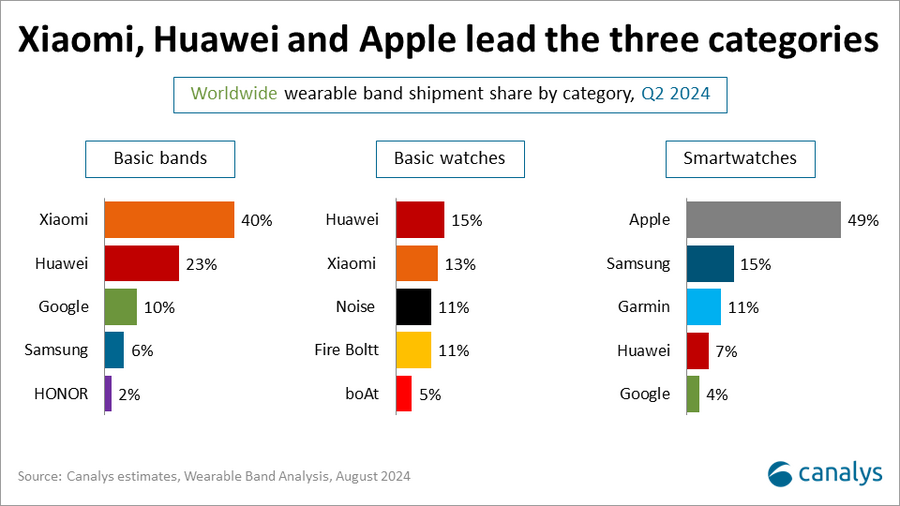
\includegraphics[width=1.0\linewidth]{./images/wearable_brand_diffusion.png}
    \caption[Wearable diffusion by major brands.]{Wearable diffusion by major brands \protect\cite{WearableDevicesBrandDiffusion}.}
    \label{fig:brandDiffusion}
\end{figure*}
\FloatBarrier

    \newpage
\section{System Specifications}
% This section of the elaborate will involve the discussion of the system requirements, as well as how the system have been designed.
\subsection{System Requirements}
By defining the system functional requirements, the application key functionalities to implement were identified, by considering also existing applications (see \cref{popularApps}) that represent standards on the health and fitness market. Security, usability as well as other important aspects were considered, leading to the definition of the non-functional requirements. The requirements can be classified as follows:
\vspace{5ex}
\begin{table}[h!]
    \setstretch{\myspacing}
    \centering
    \begin{tabular}{|>{\raggedright\arraybackslash}p{0.1\linewidth}|>{\raggedright\arraybackslash}p{0.2\linewidth}|>{\raggedright\arraybackslash}p{0.6\linewidth}|}
        \hline
        \textbf{FR1} & \multicolumn{2}{>{\centering\arraybackslash}p{0.7\linewidth}|}{\textbf{User Management}} \\
        \hline
        FR 1.1 & Registration & Allow a user to register through google or by defining his credentials. Additionally, allow an user to enter his demographics (age,sex,...) and body (height,weight,...) data when the registration is in progress. \\
        \hline
        FR 1.2 & Login Management & Allow a user to log in into his account with the methods that he had setup and allow also to change the password, including the possibility to recover it in case he forgot it.  \\
        \hline
        FR 1.3 & Account Management & Allow a user to log out from his account, delete it as well as add either google or classic credential method as login method, in case he hadn't used before.  \\
        \hline
    \end{tabular}
\end{table}


\begin{table}[h!]
    \setstretch{\myspacing}
    \centering
    \begin{tabular}{|>{\raggedright\arraybackslash}p{0.1\linewidth}|>{\raggedright\arraybackslash}p{0.2\linewidth}|>{\raggedright\arraybackslash}p{0.6\linewidth}|}
        \hline
        \textbf{FR1} & \multicolumn{2}{>{\centering\arraybackslash}p{0.7\linewidth}|}{\textbf{User Management}} \\
        \hline
        FR 1.4 & Home Page & Allow a user to visualize data regarding his steps, food, sleep and emotional state. Also allow to visualize data that exceeds the user goals differently (they visually differ from the other ones). \\
        \hline
        FR 1.5 & Learn Page & Allow the user to take lessons and then related quizzes to assess their preparation on the topic through the learn page. The user can browse the lesson and his topics, then take the corresponding test if he wants. \\
        \hline
        FR 1.6 & Health Measures Page & Allow a user to view his vital metrics by using charts organized in different tabs instead of raw values, for a better understanding. \\
        \hline
        FR 1.7 & Personal Information Page & Allow a user to edit some of his personal measures (provided at registration time) and add his activity goals, used as upper bound into the charts of the Home Page. \\
        \hline
    \end{tabular}
    \caption{Overview of Functional Requirements related to the User Management.}
\end{table}


\begin{table}[h!]
    \setstretch{\myspacing}
    \centering
    \begin{tabular}{|>{\raggedright\arraybackslash}p{0.1\linewidth}|>{\raggedright\arraybackslash}p{0.2\linewidth}|>{\raggedright\arraybackslash}p{0.6\linewidth}|}
        \hline
        \textbf{FR2} & \multicolumn{2}{>{\centering\arraybackslash}p{0.7\linewidth}|}{\textbf{Notification System}} \\
        \hline
        FR 2.1 & Notification System & Allow a user to receive notification with different frequencies to prompt him into inserting data regarding food, emotional aspect, balance capability, strenght capability. \\
        \hline
        FR 2.1 & Notification Parameters & Allow a user to receive notification based on common users parameter, but also personalized based on some personal parameter. \\
        \hline
        FR 2.2 & Body Balance Notification & Allow a user to receive notification to prompt him to insert data regarding his balance capability, such as balance test on one leg at a time or tandem walk. \\
        \hline
        FR 2.3 & Body Strength Notification & Allow a user to receive notification to prompt him to insert data regarding his strenght capability, such as number of squats, abdominals and push ups, as well as a grip strength test. \\
        \hline
        FR 2.4 & Emotional Notification & Allow a user to receive notification to prompt him to insert data regarding his emotional aspect by following the panas guidelines. \\
        \hline
        FR 2.5 & Food Notification & Allow a user to receive notification to prompt him into inserting data regarding his consumed food, with this type of notification being more frequent than the others. \\
        \hline
        FR 2.6 & Assessment & Allow a user to visualize a periodic assessment produced thanks to the data that were previously inserted. \\
        \hline
    \end{tabular}
    \caption{Overview of Functional Requirements related to the Notification System provided to the User.}
    \label{tab:fr2}
\end{table}

\begin{table}[h!]
    \setstretch{\myspacing}
    \centering
    \begin{tabular}{|>{\raggedright\arraybackslash}p{0.1\linewidth}|>{\raggedright\arraybackslash}p{0.2\linewidth}|>{\raggedright\arraybackslash}p{0.6\linewidth}|}
        \hline
        \textbf{FR3} & \multicolumn{2}{>{\centering\arraybackslash}p{0.7\linewidth}|}{\textbf{Data Management}} \\
        \hline
        FR 3.1 & Data Sources & Employing as main app data source Health Connect (Health data management and integration platform developed by Google), while still keeping Google Firebase as additional data source where needed. \\
        % Health Connect and Apple Health (Health data management and integration platforms, developed by Google and Apple respectively),
        \hline
        FR 3.2 & Health Data Source & The system must retrieve and display users' health data relating to steps and sleep on the home page, as well as their heart and lung data in health measures page. \\
        \hline
        FR 3.3 & Google Firebase Data Source & The system must retrieve and display users' health data related to emotional state and food on the home page. Also weight, waist circumference, grip, balance and strenght data are retrieved from this data sources and showed in the health measures page. Finally, profile and goals data are also fetched and showed into personal information page. \\
        \hline
        FR 3.4 & Health Data Backup & The system must add the necessary logic to perform a backup of the users's health data. \\
        \hline
    \end{tabular}
    \caption{Overview of Functional Requirements related to the Data Management.}
    \label{tab:fr3}
\end{table}

\begin{table}[h!]
    \setstretch{\myspacing}
    \centering
    \begin{tabular}{|>{\raggedright\arraybackslash}p{0.1\linewidth}|>{\raggedright\arraybackslash}p{0.2\linewidth}|>{\raggedright\arraybackslash}p{0.6\linewidth}|}
        \hline
        \textbf{FR4} & \multicolumn{2}{>{\centering\arraybackslash}p{0.7\linewidth}|}{\textbf{Admin Management}} \\
        \hline
        FR 4.1 & Admin Application & Allow the admin to use a web application in order to modify system metrics. \\
        \hline
        FR 4.2 & Login/Logout & Allow the admin to login into the web application, as well as to logout. \\
        \hline
        FR 4.3 & Notifications Parameters Edit & Allow the admin to change some of the metrics related to the notification system set up for users. \\
        \hline
        % SE FACCIAMO METTERE
        % FR 4.4 & Application Lessons & Allow the admin to manage the lessons that are provided to the users inside the application. \\
        % \hline
        % FR 4.5 & Application Quizzes & Allow the admin to manage the quizzes that corresponds to the lessons and are provided to the users inside the application. \\
        % \hline
    \end{tabular}
    \caption{Overview of Functional Requirements related to the Web Application provided to the Admin.}
\end{table}

\clearpage

\noindent As far as concerns the non-functional requirements, we can classify them as follows:

\begin{table}[h!]
    \setstretch{\myspacing}
    \centering
    \begin{tabular}{|>{\raggedright\arraybackslash}p{0.1\linewidth}|>{\raggedright\arraybackslash}p{0.2\linewidth}|>{\raggedright\arraybackslash}p{0.6\linewidth}|}
        \hline
        \textbf{NFR} & \textbf{Type} & \textbf{Description} \\
        \hline
        NFR1 & Reliability & The system should ensure at least 80\% accuracy and functionality over the course of a year. \\
        \hline
        NFR2 & Portability & The application must be capable of running on Android devices. \\
        \hline
        NFR3 & Security & Robust login mechanisms should be implemented to protect user data and limit access only to authorized individuals. \\
        \hline
        NFR4 & Usability & The application should be intuitive enough for users of all ages and skill levels, requiring minimal training. \\
        \hline
        NFR5 & Data Privacy & User data must adhere to OAUTH for secure data handling. \\
        \hline
        NFR6 & Performance & The app should smoothly load and handle user interactions within two seconds under typical conditions in order to achieve an optimal user experience. \\
        \hline
        NFR7 & Interoperability & The application should seamlessly connect with third-party platforms like Health Connect and Apple Health, maintaining data accuracy and improving functionality. \\
        \hline
        NFR8 & Localization & The app should support at least English and Italian languages, adapting content and formats (e.g., date, currency) accordingly. \\
        \hline
        NFR9 & Modularity & The app's architecture should support modular development to facilitate future updates without impacting the entire codebase. \\
        \hline
    \end{tabular}
    \caption{Overview of Non-Functional Requirements related to the system.}
    \label{tab:nfr}
\end{table}
\newpage
\subsection{System Design and Architecture}
\subsubsection{System Design}

While designing the system, the main components have been chosen in order to provide a clear and intuitive application system, as well as a robust and secure backend.
\newline For the frontend application part, cross-platform frameworks have been analyzed, having in mind the possibility to extend the application also to IOS platform. Flutter, React Native and Xamarin were considered, but Flutter has been chosen, thanks to the possibility to develop a single codebase for both Android and IOS, and also for his strong support by Google who created it, that makes it a stable and reliable system, as well as a big community and an official package repository where tons of libraries can be found. Considering the web application, among several frameworks available (like React, Angular, Vue.js) React has been chosen, given his diffusion, simplicity and modularity.   
\newline Regarding the backend part, different alternatives were considered, also based on the frontend and our requirements:
\begin{itemize}[nosep] % 'nosep' removes extra spacing between items
    \item \textbf{AWS Amplify}, set of tools and services provided by Amazon Web Services (AWS) to build secure and scalable mobile applications. It comes with a suite of services that streamline the development process, like authentication, storage, GraphQL and REST APIs as well as analytics. 
    \item \textbf{Express}, fast and minimalist web framework built on top of Node.js which is a javascript runtime.
    \item \textbf{Microsoft Azure}, cloud computing service that provides a wide range of cloud services, like analytics, storage, and networking. It allows developers to build, deploy, and manage applications through Microsoft-managed data centers.
    \item \textbf{Spring Boot}, a Java-based framework used to create stand-alone, production-grade applications, which simplifies the development of new applications by providing code and configuration through annotations.
    \item \textbf{Firebase}, comprehensive app development platform by Google that provides a variety of tools and services to help developers build high-quality apps quickly.
\end{itemize}
\newpage
\noindent Among them, Express was immediately discarded despite its simplicity, because it mainly focuses an APIs, does not provide authentication and it is not as rich of services as the others, so it does not fit our needs. Spring Boot was also discarded, given the need to setup external service for authentication (like keycloak IAM) and maintain a server where the backend could run. AWS Amplify and Microsoft Azure were also closer to our needs, but Firebase was chosen, thanks to his Flutter support and seamless integration (since bith made by Google) and thanks to the variety of services it provides: Cloud Firestore as a data source, the Authentication system, Cloud Storage system as well as a suite of analytics service to monitor the application (Analytics, Performance, Crashlytics).
% TODO: se ne parlo mettere Release Monitoring).
\subsubsection{System Core Architecture}

Focusing on the system core architecture, it can consequently be summarized as follows:
\begin{figure*}
    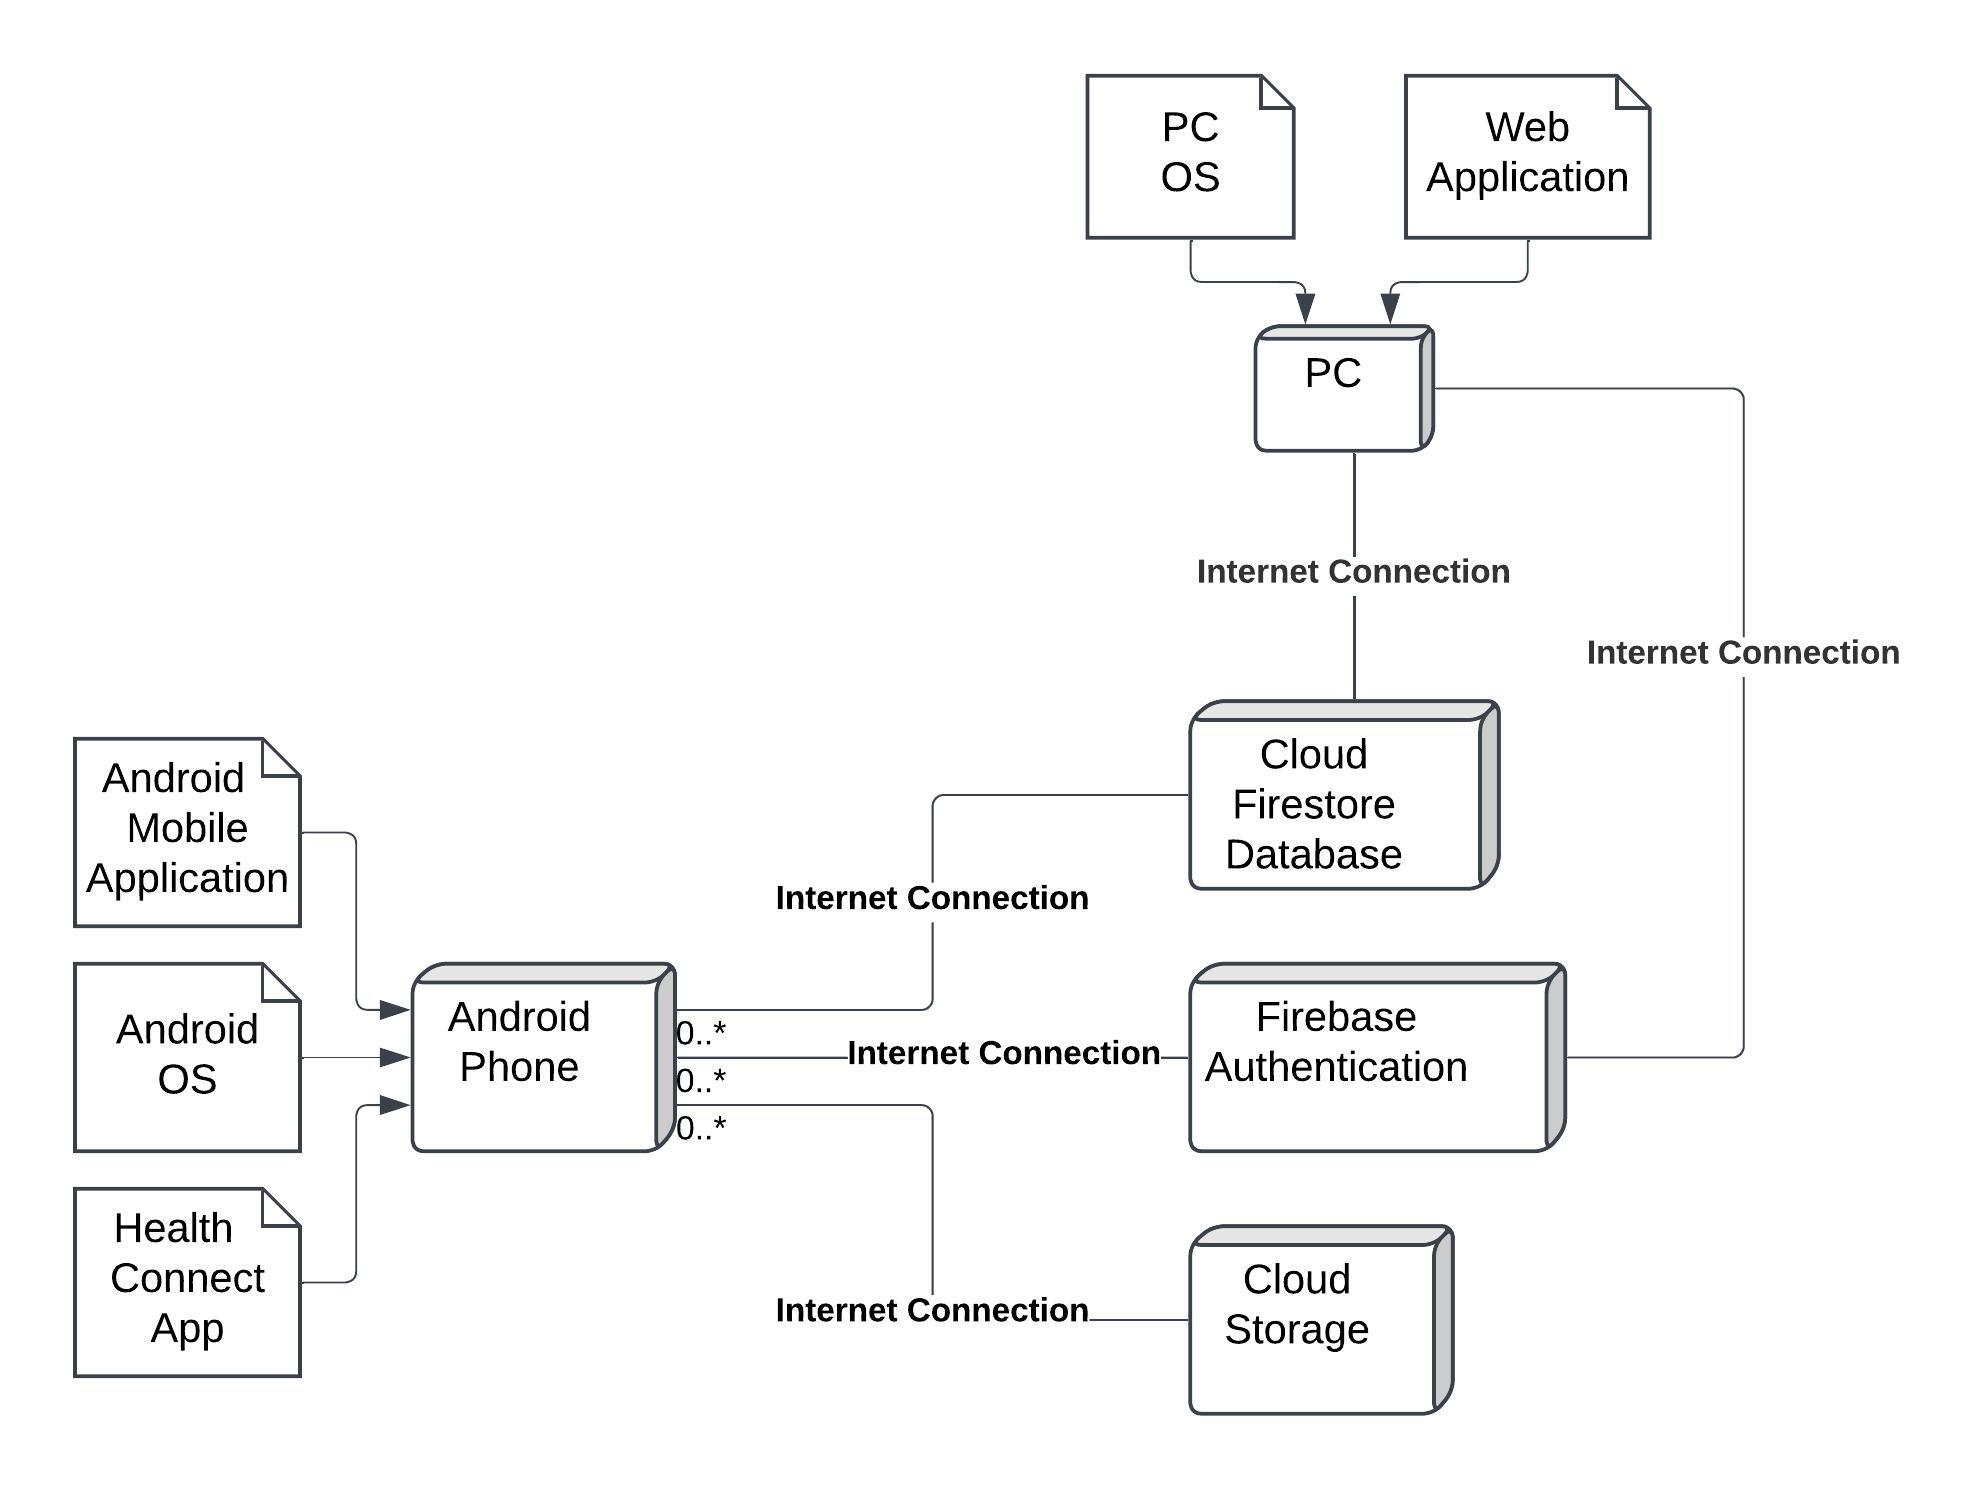
\includegraphics[width=1.0\linewidth]{./images/system_architecture.jpeg}
    \caption{Overview of the System Core Architecture.}
    \label{fig:systemArchitecture}
\end{figure*}

% \noindent We can clearly distinguish the two main use cases (Android and IOS) with their distinguishing components and the common ones:
\newpage
\noindent We can identify the core architecture with the following components:
\vspace{3ex}
\begin{itemize}[nosep] % 'nosep' removes extra spacing between items
    \item \textbf{Android Phone} that represent the physical smartphone, along with his operating system, our application installed and health connect installed, used to manage in an unified way the health data on Android.
    % , that further interacts with google fit server whenever is needed.
    % \item \textbf{Google Fit} server, used among the health connect app data sources.
    \item \textbf{Cloud Firestore Database} server, firebase service employed as a data source for the application logic, containing needed data, such as profile information.
    \item \textbf{Firebase Authentication} server, firebase service employed in order to perform and enforce authentication.
    \item \textbf{Cloud Storage} server, firebase service employed to store the backup of the health data for each user (see \cref{tab:fr3} FR 3.4).
    \item A \textbf{Personal Computer} along with his operating system and a web application that allows to authenticate and to interact with the Cloud Firestore Database on administrator side, in order to modify the system metrics for users notifications, as well as manage lessons and quizzes that are then showed to the users.  
\end{itemize}
% Firebase Performance Monitoring and Crashlytics diagnostica quindi non core
\newpage
\noindent In addition to this architecture, the system can be further enriched by integrating a wearable device, that can be a very useful tool to gather data, as previously explained in \cref{sec:wearableDevices}. In this scenario the wearable device will be connected to the smartphone:

\begin{figure*}
    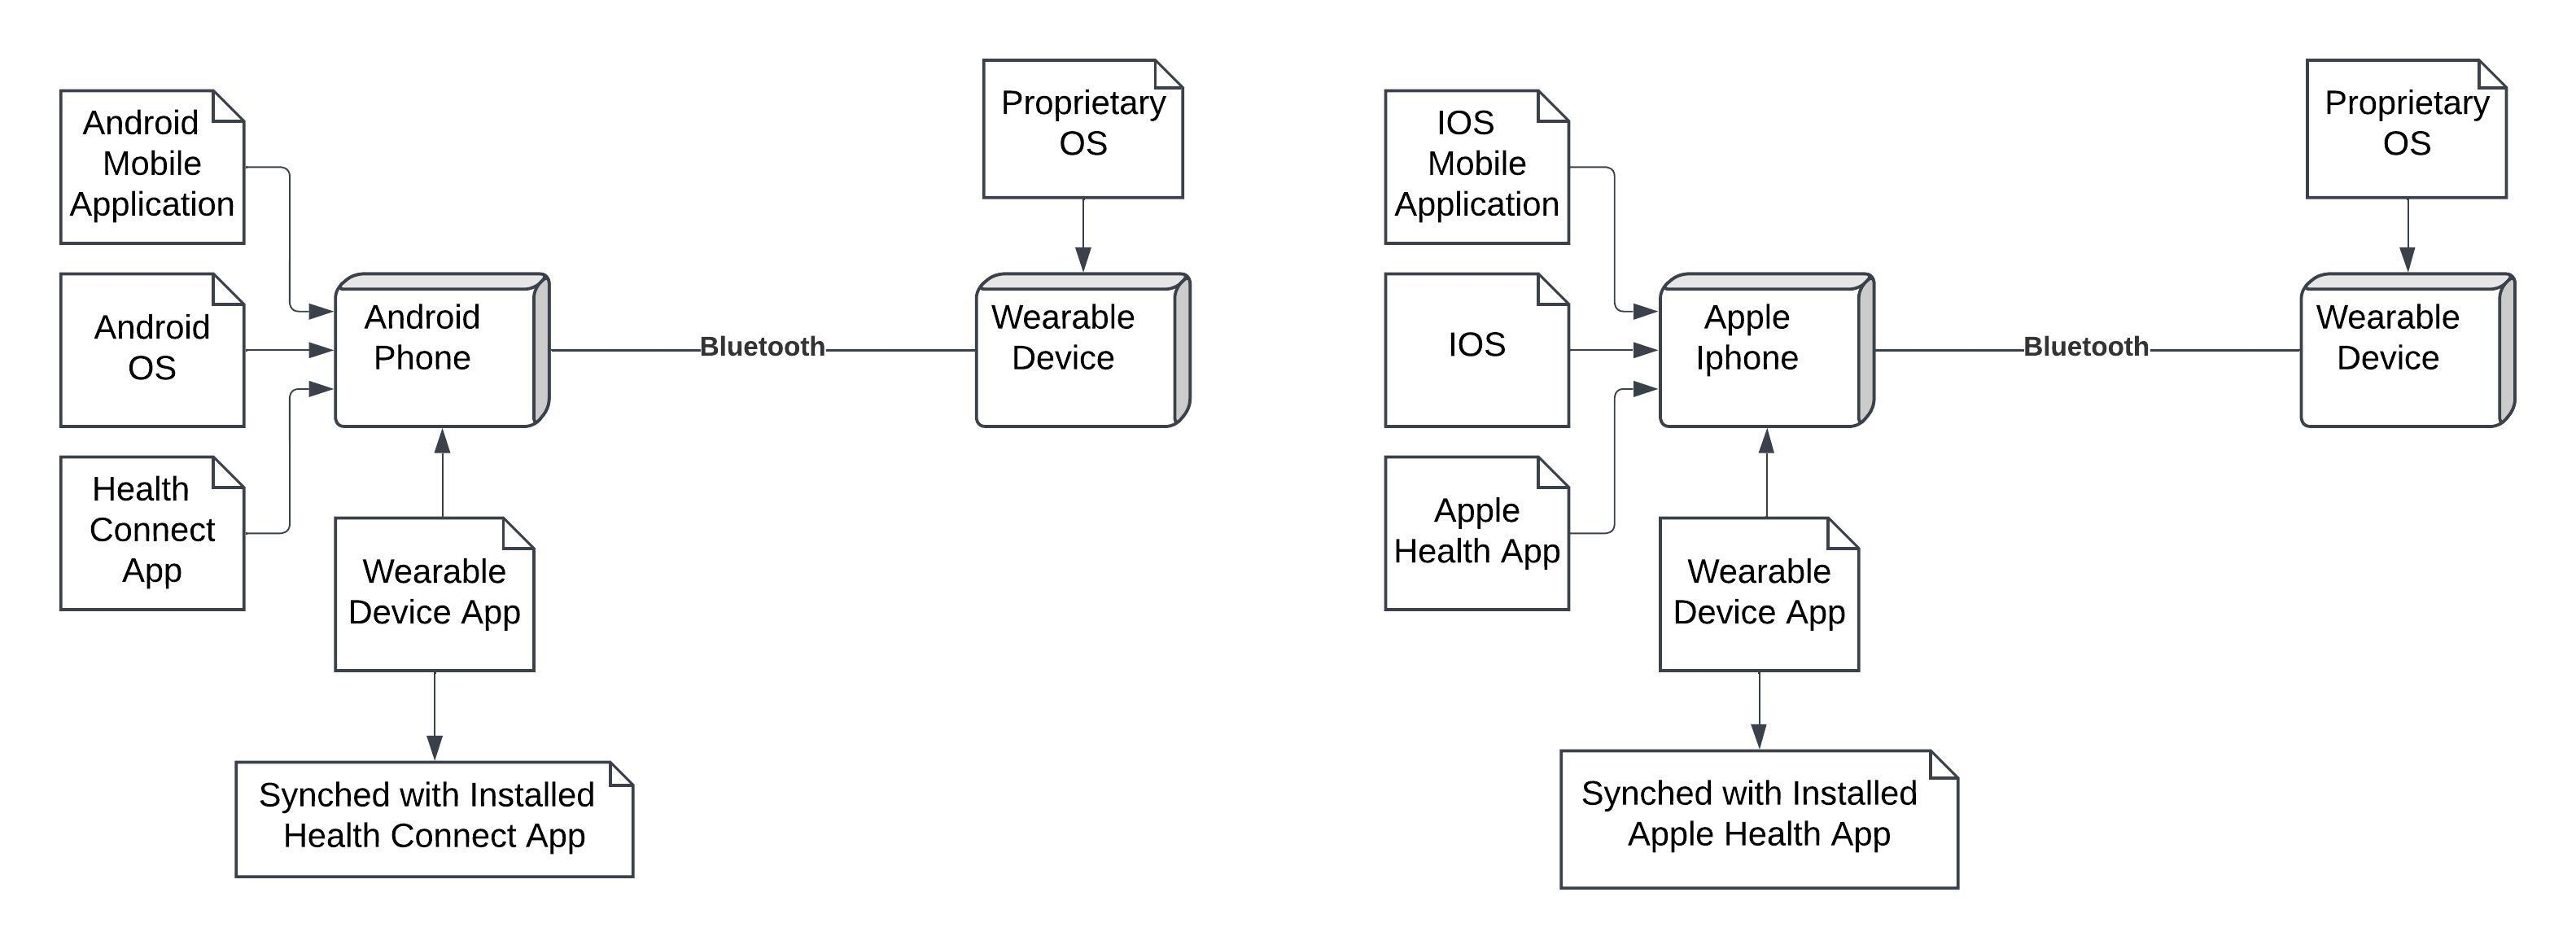
\includegraphics[width=1.0\linewidth]{./images/system_architecture_wearable.jpeg}
    \caption{Overview of the Mobile System Architecture with Wearables.}
    \label{fig:systemArchitectureWearables}
\end{figure*}

\noindent In this case the architecture has been extended with the wearable devices, along with his operating system, that through bluetooth connection can communicate with the smartphone. On the smartphone side, the wearable application will be able to retrieve the data from the wearable device to then sync with the Health Connect data management service.
% \noindent In this case the architecture has been extended with the wearable devices, along with his operating system, that through bluetooth connection can communicate with the smartphone (Android or IOS). On the smartphone side, the wearable application will be able to retrieve the data from the wearable device to then sync with the respective data management service (respectively Health Connect or Apple Health).
\newpage
    \section{Contribution}
    \section{App Implementation}
% Flutter state management spostato più in alto essendo backend posso dire
\subsection{Firebase}
\subsubsection{Firebase Authentication}
\subsubsection{Cloud Firestore Database}
\subsubsection{Cloud Storage}

\subsection{Data Visualization}
\subsubsection{Health Data Visualization}
\subsubsection{Database Data Visualization}

\subsection{Health Data Backup}
\subsection{Notifications}
\subsubsection{Notification Parameters Editing}
\subsection{MultiLanguage}
\subsection{Lessons and Quiz}
\subsubsection{Lessons and Quiz Parameters Editing}
\newpage
    \section{System Outcomes and Enhancements}

\subsection{Achieved Performances}

\subsection{Future Developments}
Ios integration
Large Language Model (spiegare che il backup per questo è stato fatto per addestrare in futuro llm)
    % REMOVE TO USE DEFAULT BIBLOGRAPHY FONT SIZE
\defbibheading{bibliography}{%
  \newpage
  \phantomsection % Ensures the correct link location
  \section*{\headerFont{Bibliography}} % Customize the size and title here
  \singlespacing
}

\phantomsection % Ensures the correct link location
\printbibliography
\addcontentsline{toc}{section}{Bibliography} % Adds Bibliography to ToC

\begingroup
  \newgeometry{top=0cm,left=\myleftmargin,right=\myrightmargin} % Set custom margins for the LoF
  % Custom command to display the List of Figures
  \begin{spacing}{\myspacing}
    \begingroup
      \phantomsection % Create anchor for ToC entry
      \addcontentsline{toc}{section}{\itemFont{List of Figures}} % Adds List of Figures to ToC with custom formatting
      \renewcommand{\listfigurename}{\headerFont{List of Figures}}
      \renewcommand{\addtocontents}[2]{} % hide the default one
      \listoffigures % Generates the List of Figures but does not add it to the ToC
    \endgroup
  \end{spacing}
\endgroup
% To have good margin on the second page of the list of figures
\clearpage
\newgeometry{top=\mytopmargin,left=\myleftmargin,right=\myrightmargin} % Adjust top margin for the second page

\restoregeometry
    \newpage
\pagestyle{empty}
\begin{spacing}{\myspacing}
\section*{Ringraziamenti}

Pensare al percorso che ho fatto in questi anni, così come tutte le persone che hanno contribuito a renderlo tale, mi rende felice e un pizzico nostalgico. Se sono arrivato qui, oltre che a me stesso, lo devo a tutte queste persone.
\vspace{2ex}
\newline \noindent Ringrazio il mio relatore, Prof. Maurizio Morisio, per la sua disponibilità e il suo sostegno durante il tirocinio e la tesi.
\vspace{2ex}
\newline \noindent Ringrazio i miei genitori, Gaetano e Maria, per tutti i sacrifici che hanno fatto, e che mi hanno permesso di arrivare dove sono. Senza il loro aiuto non sarei certamente qui ora.
\vspace{2ex}
\newline \noindent Ringrazio i miei nonni Vincenza, Domenico, Sofia e Santino, per il loro supporto e amore incondizionato.
\vspace{2ex}
\newline \noindent Ringrazio i miei zii e cugini per il loro supporto e affetto dimostratomi. 
\vspace{2ex}
\newline \noindent Anche se non coinvolti con l'università, vorrei ringraziare i miei amici più stretti per la loro preziosa compagnia: Vincenzo Petrillo, amico d'infanzia di una vita, ma anche Alberto Contaldi per la sua follia e Giuseppe Romano.
% \newline \noindent Even if not involved with actual projects, I would like to thank my other closest friend for their company during this experience: \textbf{Vincenzo Petrillo}, childhood friend of a lifetime, but also \textbf{Alberto Contaldi} (known as the \textbf{leccapali}) with his madness and \textbf{Giuseppe Romano} (known as the \textbf{tozzo sicario con presa a sigaro}).  
\vspace{2ex}
\newline \noindent Ringrazio i miei colleghi e amici:

\begin{itemize}[nosep] % 'nosep' removes extra spacing between items
    \item Gaetano, noto anche come Tanucc/TanoDev, per tutte le risate e i momenti di studio e divertimento condivisi.
    \item  Alessandro, noto anche come la Regina Regale, per la sua presenza regale durante i momenti di studio e divertimento, e tutte le risate condivise.
    \item Davide, noto anche come DaveBreaks, per i tanti momenti di divertimento condivisi insieme (non di studio dal momento che mi ha torturato con la grammatica e il padding [\texttt{187.92 px} numero perfetto], ma lo voglio bene lo stesso).
    \item Vorrei anche ringraziare Giorgio e Giuseppe (noto anche come LoHacker) per la loro compagnia e le tante risate condivise.
\end{itemize}
\vspace{2ex}
\noindent Insieme abbiamo condiviso la maggior parte dei giorni di studio, e li ringrazio per averli resi meno faticosi e certamente più divertenti, tra una risata e l'altra. Abbiamo condiviso tutta la difficoltà di questo corso, e siamo riusciti a superarla insieme.
\vspace{2ex}
\newline \noindent Ringrazio tutti voi con i quali ho condiviso una parte di me e del mio percorso.
\end{spacing}
% \newpage
% \pagestyle{empty}
% \begin{spacing}{\myspacing}
% \section*{Acknowledgements}

% Thinking about the journey I have made in those years, as well as all the people who helped make it so, makes me very excited and leaves me speechless. If I got here, besides myself, I owe it to all these people.
% \newline \noindent I thank my supervisor, Prof. Maurizio Morisio, for his availability and his support during the internship and thesis.
% \newline \noindent I thank my parents, Gaetano and Maria, for all the sacrifices they have made, and that allowed me to get where I am. Without their help I would certainly not be here now.
% \newline \noindent Even if not involved with university and actual projects, I would like to thank my closest friend for their precious company: Vincenzo Petrillo, childhood friend of a lifetime, but also Alberto Contaldi for his madness and Giuseppe Romano.
% % \newline \noindent Even if not involved with actual projects, I would like to thank my other closest friend for their company during this experience: \textbf{Vincenzo Petrillo}, childhood friend of a lifetime, but also \textbf{Alberto Contaldi} (known as the \textbf{leccapali}) with his madness and \textbf{Giuseppe Romano} (known as the \textbf{tozzo sicario con presa a sigaro}).  
% \newline \noindent I thank my colleagues and friends: 

% \begin{itemize}[nosep] % 'nosep' removes extra spacing between items
%     \item Gaetano, also known as Tanucc/TanoDev, for all the laughs and moments of study and fun shared together. 
%     \item Alessandro, also known as the Regal Queen, for his regal presence during many moments of study and fun, and all the laughs shared together.
%     \item Davide, also known as DaveBreaks, for the many moments of fun shared together (not of study since he tortured me with the grammar and the padding, but I still love him).
%     \item I would also like to thank Giorgio and Giuseppe (also known as LoHacker) for their company and the many laughs shared together.
% \end{itemize}
% \vspace{2ex}
% \noindent Together we shared most of the study days, and I thank them for making it less strenuous, and certainly more fun, between one laugh and the other. We also shared all the effort and difficulties of this course, and we managed to overcome them together. 
% \newline \noindent I thank all of you with whom I have shared a part of myself and my journey.
% \end{spacing}
\end{spacing}

\end{document}
